% This is samplepaper.tex, a sample chapter demonstrating the
% LLNCS macro package for Springer Computer Science proceedings;
% Version 2.21 of 2022/01/12
%
\documentclass[runningheads]{llncs}
%
\usepackage[T1]{fontenc}
% T1 fonts will be used to generate the final print and online PDFs,
% so please use T1 fonts in your manuscript whenever possible.
% Other font encondings may result in incorrect characters.
%
\usepackage{graphicx}
% Used for displaying a sample figure. If possible, figure files should
% be included in EPS format.
%
% If you use the hyperref package, please uncomment the following two lines
% to display URLs in blue roman font according to Springer's eBook style:
%\usepackage{color}
%\renewcommand\UrlFont{\color{blue}\rmfamily}
%\urlstyle{rm}
%

% Olivier
\usepackage{changepage}
\usepackage{amssymb}
% \newcommand{\doublecheck}{\stackon{\checkmark\hspace{-0.3em}}{\checkmark}}
\newcommand{\doublecheck}{\checkmark\hspace{-0.5em}\checkmark}

\usepackage{subcaption}

\usepackage{ulem}

%%%%%%%%%%%%%%%%%%%%%%%%%%%%%%%%%%%%%%%%%%%%%%%%%%%%%%%%%

\begin{document}
%
\title{Schema Mechanisms 2.0 for Developmental Artificial Intelligence}
%
\titlerunning{Schema Mechanisms 2.0}
% If the paper title is too long for the running head, you can set
% an abbreviated paper title here
%
\author{Olivier~L.~Georgeon\inst{1}\orcidID{0000-0003-4883-8702} \and
Filipo~S.~Perotto\inst{2}\orcidID{0000-0003-2283-4703} \and
Kristinn~R.~Th{\'o}risson\inst{3}  \and
Arash~Sheikhlar\inst{3} \and
Paul~Robertson\inst{4}\orcidID{0000-0002-4477-0379}
}
%
\authorrunning{Georgeon, Perotto, Th{\'o}risson, Scheikhlar, \& Robertson}
% First names are abbreviated in the running head.
% If there are more than two authors, 'et al.' is used.
%
\institute{UR CONFLUENCE: Sciences et Humanites (EA 1598), UCLy, France \email{ogeorgeon@univ-catholyon.fr}\\
\and ONERA -- The French Aerospace Lab -- DTIS, Toulouse, France \email{filipo.perotto@onera.fr}
\and Center for Analysis and Design of Intelligent Agents, Reykjavik University, Iceland \email{thorisson@ru.is}, \email{arash@iiim.is}
\and DOLL Labs, Lexington, MA, USA\\ \email{paulr@dollabs.com}
 }
%
\maketitle              % typeset the header of the contribution
%
\begin{abstract}
Schema mechanisms are software frameworks designed to reflect learning theories like genetic epistemology, constructivist epistemology, and developmental learning.
Building on Gary Drescher’s pioneering implementation from 1991, this paper reviews four contemporary schema mechanisms: CALM, LIDA, ECA, and AERA. 
While maintaining Drescher’s Piagetian-inspired view that sensorimotor schemas serve as the foundation for knowledge construction, these new mechanisms extend the constructivist approach by grounding schemas in interactional events rather than static world perceptions. 
This shift introduces an interactional motivation framework and integrates hierarchical abstraction, internal simulation, and physical space into schemas, paving the way for their application in autonomous robotics operating in open environments. 
We believe that these advancements mark the emergence of a new generation of schema mechanisms, which we refer to as Schema Mechanisms 2.0.



%Gary Drescher pioneered their implementation in 1991, laying the foundation for the field of Constructivist AI.
%and identified the core challenges: open-ended learning, intrinsic motivation, discovering of empirical regularities, incremental hierarchical abstraction, concept invention, sensorimotor grounding, reflexivity, individuation. 

%The central body of reference of these theories is found in the work of Jean Piaget ranging from theory of knowledge to child psychology, and 
%These theories find roots in the work of Jakob von Uexküll on animal behavior, Ernst von Glasersfeld on epistemology, and, more centrally, Jean Piaget ranging from child psychology to theory of knowledge.
%Gary Drescher coined the generic term schema mechanism and pioneered their implementation in 1991.
%FP: fix the phrase "His work laid the ground to identifying the core challenges:" 
%FP: add "creation of concepts" and "detection of regularities during interaction" in the challenges list

%His work laid the ground in the Constructivist AI field and identified the core challenges: open-ended learning, intrinsic motivation, discovering of empirical regularities, incremental hierarchical abstraction, concept invention, sensorimotor grounding, reflexivity, individuation. 
%he modeled Piagetian sensorimot schemas as datastructures that encompass sensory data and actions, 
%FP: the latest schema mechanisms 
%schema mechanisms from the literature, and highlights their contributions to these key challenges, with the goal of unifying their different contributions toward a comprehensive theory of developmental artificial intelligence.


\keywords{schema mechanism  \and genetic epistemology \and constructivist learning \and intrinsic motivation \and cognitive architectures.}
\end{abstract}
%
%%%%%%%%%%%%%%%%%%%%%%%%%%%%%%%%%%%%%%%%%%%%%%%%%%%%%%%%%%%%%%%%%%%%%%%%%%%%%%%%%%%%%%%%%%%%
%
\section{Introduction}
\label{sec:intro}
%
% Drawing from the earlier work of James Baldwin, 
Throughout his life, Jean Piaget developed and popularized the theory of \textit{genetic epistemology} \cite{piaget_principles_1997}  to account for the genesis of intelligence and knowledge. 
In parallel, he pioneered \textit{developmental psychology} by establishing the foundational methods for studying mental development in children~\cite{piaget_origins_1955,piaget_reality_1955}.
Toward the end of his life, he connected genetic epistemology with constructivist epistemology and the work of Ernst von Glasersfeld \cite{glasersfeld_radical_1997}. 
Genetic epistemology rests on the key concept of ``schema'', closely related to the concept of ``functional circles'' proposed by Jakob von Uexküll.
We refer to Ziemke \cite{ziemke_construction_2001} for a broader discussion on the philosophical roots of constructivist epistemology in Kant's philosophy, and Uexküll's biology.  
Piaget defines a schema as follows: 
\\

\begin{adjustwidth}{1cm}{1cm}
%``A schema is a structure or organization of actions as they transfer or generalize in similar or analogous circumstances.''
``A schema is a structure or organization of actions as they are transferred or generalized by repetition in similar or analogous circumstances.''
%(\cite{piaget_naissance_1998}, p. 23).
(\cite{piaget_psychology_1969}, p.~4).
\\ 
\end{adjustwidth}

%FP: simply use schema, it is done in every english version of Piaget books
%In this paper, we translate the French term \textit{scheme} with the English term \textit{schema} and we use the plural \textit{schemas}. 
A schema is the basic unit of knowledge that encapsulates an action and its circumstances, that is, a \textit{pattern of interaction}. 
Genetic epistemology insists on the primacy of interaction as a condition for the emergence of perception and knowledge, 
%FP: add
surpassing innatist and empiricist explanations:
\\

\begin{adjustwidth}{1cm}{1cm}
``Knowledge does not originally arise either from a subject conscious of itself or from objects already constituted (from the subject's point of view) that would impose themselves on the subject. 
Knowledge results from interactions occurring halfway between the subject and the objects, and thus involving both, but due to a complete un-differentiation and not from exchanges between distinct forms.

If, at the beginning, there is neither a subject, in the epistemic sense of the term, nor objects, conceived as such, nor, above all, invariant instruments of exchange, then the initial problem of knowledge will be to construct such mediators. 
Starting from the contact zone between one's own body and the objects, these mediators will progressively engage more deeply in both complementary directions toward the exterior and the interior. 
It is from this dual progressive construction that the joint elaboration of both the subject and the objects depends.

The initial instrument of exchange is not perception, as rationalists too easily conceded to empiricism, but rather action itself, with its much greater plasticity. 
Certainly, perceptions play an essential role, but they partly depend on action as a whole, and some perceptual mechanisms that one might have thought to be innate or very primitive only emerge at a certain level of object construction.'' (translated from \cite{piaget_lepistemologie_2011}, p.~14-15)
\\

\end{adjustwidth}

For Piaget, intelligence is related to the ability to gradually organize and complexify the set of schemas. 
Increasing organization of internal structures are guided by two forces: 
by assimilating new experiences to existing schemas, the mind tries to integrate observations and interactions in terms of already constructed cognitive structures, extending or generalizing their scope, and
by accommodating its set of schemas to surprising or disruptive experiences, differentiating, specializing, complexifying its internal relations, the mind creates new intellectual resources for better understanding and mastering its interactions: 
\\

\begin{adjustwidth}{1cm}{1cm}
``[...] Organization is inseparable from adaptation: they are two complementary processes of a single mechanism, organization being the internal aspect of the cycle of which adaptation constitutes the external aspect. [...] that adaptation is an equilibrium between assimilation and accommodation. [...] Intelligence is assimilation to the extent that it incorporates all the given data of experience within its framework. [...] That mental life is also accommodation to the environment. Assimilation can never be pure because by incorporating new elements into its earlier schemata the intelligence constantly modifies the latter in order to adjust them to new elements.''~(\cite{piaget_origins_1955}, p.~7)

``In their initial directions, assimilation and accommodation are obviously opposed to one another, since assimilation is conservative and tends to subordinate the environment to the organism as it is, whereas accommodation is the source of changes and bends the organism to the successive constraints of the environment. But if in their rudiment these two functions are antagonistic, it is precisely the role of mental life in general and of intelligence in particular to intercoordinate them.''~(\cite{piaget_reality_1955}, p.~352)

``Gradually, as the child's thought evolves, assimilation and accommodation are differentiated and become increasingly complementary. 
In the realm of representation of the world this means, on the one hand, that accommodation, instead of remaining on the surface of experience, penetrates it more and more deeply, that is, under the chaos of appearances it seeks regularities and becomes capable of real experimentations to establish them. 
On the other hand, assimilation, instead of reducing phenomena to the concepts inspired by personal activity, incorporates them in the system of relationships rising from the more profound activity of intelligence itself.''~(\cite{piaget_reality_1955}, p.~385)

``The study of sensorimotor or practical intelligence in the first two years of development has taught us how the child, at first directly assimilating the external environment to his own activity, later, in order to extend this assimilation, forms an increasing number of schemata which are both more mobile and better able to intercoordinate.
[...] The increasing coherence of the schemata thus parallels the formation of a world of objects and spatial relationships, in short, the elaboration of a solid and permanent universe.''~(\cite{piaget_reality_1955}, p.\textit{xi})
\\

\end{adjustwidth}

Schema mechanisms attempt to reflect the key insights of genetic epistemology effectively expressed by these words of Piaget regarding the primary role of sensorimotor experience and organization of mental structures. 
Indeed, genetic epistemology appears to provide a materialistic explanation of how the human mind develops from birth, potentially lending itself to computational implementation.

Over the past decades, Piaget's theories have remained central to contemporary theories of knowledge development, continually questioned and shaped by active debates.
Some shortcomings have been identified, including an underestimation of infants' abilities and an insufficient consideration for cultural and social factors (e.g., \cite{soran_university_piagets_2019}).
The relationship between constructivist and nativist theories remains a topic of debate, raising questions about the innate knowledge and prerequisites that should be incorporated into any computational implementation \cite[p. 41]{drescher_made-up_1991}.
The ongoing research on schema mechanisms examined in this paper contributes to these debates.





%To this day, nonetheless, Piaget's ideas remain central to modern theories of knowledge as well as developmental psychology. 

%FP: suggestion, we can maybe cut out this last phrase? but you can undone my modification if you like it in this way  :)
%\sout{To our knowledge, Piaget never claimed that his theories could be implemented as a mechanistic process in a computer. 
%The first attempt only began eleven years after his death.}

%FP:
%*** What to do with this references? \cite{chaput_constructivist_2004,guerin_piagetian_2008,miller_building_2018} ***


%%%%%%%%%%%%%%%%%%%%%%%%%%%%%%%%%%%%%%%%%%%%%%%%%%%%%%%%%%%%%%%%%%%%%%%%%%%%%%%%%%%%%%%%%%%%
%
\section{Schema mechanisms}
\label{sec:schema}
%
Implementing genetic epistemology as a mechanistic process involves reducing Piaget's psychological concept of schema into data structures handled by a computer. 
This computer controls an artifact (robot or virtual agent) that interacts with its environment.
The computer must process these data structures through some mechanism that will support the generation of increasingly intelligent behavior demonstrating the internal development of the robot.
Guerin and McKenzie \cite{guerin_survey_2013} proposed the graphical representation of this developmental process shown in the Figure~\ref{fig:general}.
%
\begin{figure}
	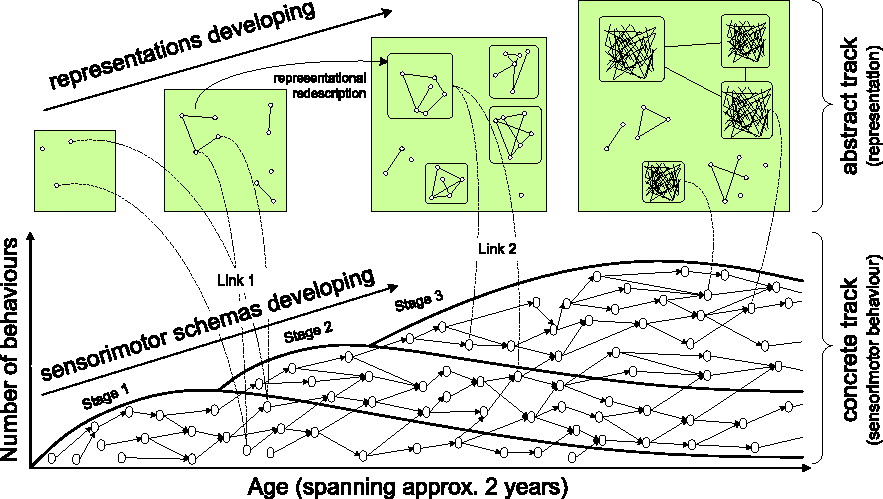
\includegraphics[width=\textwidth]{Figure_1_guerin.pdf}
	\caption{Conceptual diagram of infant development from \cite{guerin_survey_2013} Fig. 1.
	The lower (concrete) track shows a directed acyclic graph of sensorimotor schemas. 
	A node represents a newly created schema. 
	An edge has the meaning ``is a necessary precursor''. 
    Stage 1: behaviors without objects. 
    Stage 2: behaviors with single objects. 
    Stage 3: object-object behaviors. The schemas now involve relationships among objects, and locations and transforms within space.
    The higher (abstract) track represents representations of objects by schemas and physical properties influencing their interactions.} 
	\label{fig:general}
\end{figure}

Notably, the developmental process is not targeted at reaching a predefined goal-state in a predefined problem space, nor does it aim at maximizing a predefined scalar value as in reinforcement learning.
Instead, the problem of cognitive development in artificial systems is intertwined with the problem \textit{intrinsic motivation}, as has been argued for example by  
Oudeyer and colleagues \cite{oudeyer_intrinsic_2007}. 

%%%%%%%%%%%%%%%%%%%%%%%%%%%%%%%%%%%%%%%%%%%%%%%%%%%%%%%%%%%%%%%%%%%%%%%%%%%%%%%%%%%%%%%%%%%%

\subsection{Drescher's Schema Mechanism}
%\subsection{Marginal Attribution and Representation Construction System (MARCSYST)}

In the early 1990s, Gary Drescher pioneered the first schema mechanism as a result of his PhD thesis~\cite{Drescher:1989} and associated publications~\cite{Drescher:1987,Drescher:1993}, which gave rise to a successful book~\cite{drescher_made-up_1991}, proposing a framework to reproduce key constructivist notions in artificial intelligence.
%, and presenting an implemented mechanism called \textit{Marginal Attribution and Representation Construction System} (MARCSYST).
%Drescher notes that ``a constructivist account of the development of intelligence holds that the difference between the mind of an adult, and that of an infant, lies in mental structures built by the individual'' \cite[p. 41]{drescher_made-up_1991}.
%He pioneered the first schema mechanism in 1991 by designing 
%In his work, these mental structures are designed as schemas, 
Drescher formalized schemas as the tuple $\langle \textit{context}, \textit{action}, \textit{result} \rangle$ depicted in Fig. \ref{fig:drescher}.
The \textit{context} and the \textit{result} are sets of binary \textit{items} that can be \textit{positively} or \textit{negatively} included. 
A schema's context is satisfied when all the positively included items are \textit{On} and all the negatively included items are \textit{Off}. 
A schema's result asserts that, if the \textit{action} is taken when the context is satisfied, then the positively included items of the results will be turned \textit{On} and its negatively included items will be turned \textit{Off}.

\begin{figure}
	\centering
	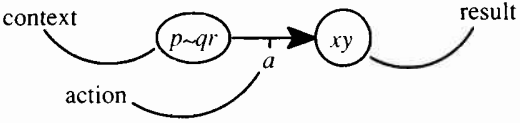
\includegraphics[width=0.6\textwidth]{Figure_2_schema_drescher.png}
	\caption{Schema from \cite{drescher_made-up_1991} Fig. 3.2.
		The schema noted $p \!\sim\! qr/a/xy$ asserts that if action $a$ is taken in the context where item $p$ is On, $q$ is Off, and $r$ is On then the items $x$ and $y$ will be turned On.} 
	\label{fig:drescher}
\end{figure}

The agent is initialized with a set of \textit{primitive} items and actions that represent builtin elementary sensorimotor variables. 
For each primitive action, a \textit{bare schema} with empty context and result is created. 
The designer may also add other initial schemas that encode the agent's ``innate'' behaviors. 
%The agent is initialized with a set of \textit{primitive} ivactions and items, that represent respectivelly builtin elementary sensorimotor variables, and with a population of initial schemas, some of them are \textit{bare schemas}, one for each primitive action, with empty context and result, and eventually other initial schemas that encode the agent's initial ``innate'' behaviors. 

The \textit{activation} of a schema consists of initiating its action. 
Upon completion of the action, the predicted result is compared with the actual result.
The schema is said to \textit{succeed} if its predicted results are all obtained, and to \textit{fail} otherwise. 
The ratio of success and failure is called \textit{reliability} and is memorized for each schema.  
%As the agent interacts with its environment, it records new schemas that associate the observed context together with the action taken and the observed result. 

%Drescher implemented Piaget's idea of ``construction of reality'' through a mechanisms that seeks underlying invariant that make the enaction of some schemas reliable. 
The learning of new schemas is triggered by the identification of \textit{relevant results} made of items that are slightly more frequent than average. 
When a relevant result is identified, the agent seeks conditions under which it follows reliably. 
Such conditions are found through new schemas that allow recovering the context leading to the relevant result, and then performing the action again to asses the reliability of these new schemas. 

After learning new schemas, the agent can learn new ``concepts'' when it identifies schemas that act as ``probes'' that may evoke the manifestation of a ``thing''. 
These schemas are only reliable if the ``thing'' is present. 
When such a schema is found, it is considered a \textit{host schema} for a newly spawned \textit{synthetic item} that represents this thing.
Eventually, the agent finds out that a single ``thing'' may manifest itself through different host schemas. 
Drescher notes that ``a synthetic item thus works backward from a thing's manifestation to define the very thing manifested'' \cite[p. 83]{drescher_made-up_1991}.
This addresses the fundamental problem of \textit{concept invention} in that 
``a synthetic item is a new element of the system's ontology---an element fundamentally different from the prior contents of the system's conceptual vocabulary'' \cite[p. 81]{drescher_made-up_1991}.

The designer defines the agent's goals by assigning \textit{primitive values} (positive if desirable, negative if dreaded) to values of items (\textit{On} or \textit{Off}).
The mechanism can identify subgoals as specific sets of items to be activated or deactivated; 
and it constructs \textit{composite actions} as sequences of schemas used to reach a subgoal.
The values of a target item may be propagated to other items in the form of \textit{instrumental values} and \textit{delegated values} when attaining these other items improves the chances to reach the target item. 
%Items also have \textit{instrumental values} and \textit{delegated values} that enter into play in the selection of schemas and composite actions.
%Schemas can be combined and chained to form \textit{composite actions} that serve to reach desirable goal states. 
The agent randomly alternates between explicit goal-pursuit and exploration, with probability defined by the designer.

%Drescher targeted the fundamental problem of \textit{concept invention} by implementing a mechanism to find underlying invariant 

%The new synthetic item is created in terms of primitive or previously created synthetic items.
%For example, returning the hand to where an object was last felt typically recovers the tactile manifestation of the object. A new concept is learned to represent this object. 

%This processes uses the mechanism's \textit{marginal attribution} facility, which ``use[s] sensitive statistical measures to alternate between discovering a highly unreliable result, and then seeking conditions with respect to which the result follows more reliably'' \cite[p. 5]{drescher_made-up_1991}.

% New items called \textit{synthetic items} are learned through a process called \textit{marginal attribution}.

Drescher demonstrates its schema mechanism in the ``microworld'' made of the two-dimensional grid shown in Fig. \ref{fig:drescher2}.
``The mechanism controls a simulated robot that has a body, a single hand, and a visual system. 
The hand can touch and grasp objects, and move them about.
The visual system maps a visual field onto a region of the world in the immediate vicinity of the robot body'' \cite[p. 114]{drescher_made-up_1991}. 

\begin{figure}
	\centering
	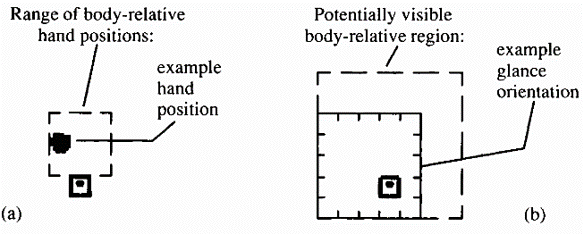
\includegraphics[width=0.6\textwidth]{Figure_drescher_expe.png}
	\caption{Drescher's benchmark from \cite[Fig. 6.1]{drescher_made-up_1991}. The simulated robot's body is represented by the small square with a black dot. 
		(a): The hand (black spot) can move in the $3 \times 3$ grid in front of the body.
		(b): The visual field is the $5 \times 5$ grid in the environment made of a $7 \times 7$ grid.} 
	\label{fig:drescher2}
\end{figure}

The mechanism initially ignores the topological relations among sensory items, but the demonstration shows that it gradually learns these relations in a process that Drescher calls the ``elaboration of the spatial substrate''. 
Such learning of a cognitive map from sensorimotor sequences has recently been further investigated by Raju et al. \cite{raju_space_2022}.

Once the spatial substrate is learned, the mechanism manages to construct synthetic items that designate objects as distinct from their current perceptions.
Drescher gives the example of ``a synthetic item, which we might call \texttt{PalpableObjectAt(1,3)} (the name, of course, has no meaning to the mechanism). 
The item is defined to represent whatever condition makes the schema reliable; we observers know (but the mechanism does not) that this condition is that there be an object at (1, 3)'' \cite[p. 13]{drescher_made-up_1991}.
Synthetic item \texttt{PalpableObjectAt(1,3)} may later be associated with \texttt{VisibleObjectAt(1,3)} to account for the discovery that they refer to the same thing at position (1, 3) in the world.

In summary, Drescher's schema mechanism stands among the first attempts to investigate Piaget's question of how the child's mind can dynamically construct its own knowledge of reality from experience of interaction.  
In our view, Drescher's main contribution to this question rests on the construction of synthetic items to account for ``things in the world'' that the agent can discover through regularities in sequences of sensorimotor experience. 
Drescher goes beyond his predecessors (e.g., \cite{harnad_symbol_1990}) who merely categorized passively-received inputs.
His schema mechanism was the first that ``grounds its synthetic items in the reification of counterfactual assertions'' \cite[p. 90]{drescher_made-up_1991}. 

Drescher identified some limitations that may explain why nobody has made his mechanism work in a more complex environment since its creation almost 40 years ago. 
These limitations follow from the acknowledgment that ``whatever experiences an organism or mechanism has had, there are infinitely many mutually contradictory generalizations that are consistent with those experiences. 
Therefore, any induction apparatus must impose a choice among those consistent generalizations'' \cite[p. 174]{drescher_made-up_1991}.
%Among these choices, he acknowledges that ``looking for persistence is built into the schema mechanism's synthetic item facility; thus, the significance of persistence is innate to the mechanism, rather than being acquired'' \cite[p. 84]{drescher_made-up_1991}.

Due to specific design choices, Drescher's schema mechanism may lack generality.
For example the assumption that a sensory item ``is a state element'' and ``each item represents some condition in the world'' \cite[p. 56]{drescher_made-up_1991} presupposes that the world is defined as a predefined set of states, which is acceptable in a microworld but difficult in the physical world. 
Another assumption was to model the agent's motivation through positive and negative values associated with sensory items.
%FP: "representing elements of the world." in fact Drescehr does not suppose that the items represent elements of the external world - they can be proprioceptive.
The exploration mechanism based on hysteresis and habituation may also lack generality;  
other motivational principles can be imagined. 
Conversely, a schema mechanism may need additional built-in assumptions to cope with the complexity of the physical world.
This paper reviews other schema mechanisms that make other choices in the hope to move forward towards a general schema mechanism that could work in the real world.

%%%%%%%%%%%%%%%%%%%%%%%%%%%%%%%%%%%%%%%%%%%%%%%%%%%%%%%%%%%%%%%%%%%%%%%%%%%%%%%%%%%%%%%%%%%%

%\subsection{Perotto's}
\subsection{Constructivist Anticipatory Learning Mechanism (CALM)}

In the early 2010s, Filipo S. Perotto proposed his own version of a schema mechanism, called \textit{Constructivist Anticipatory Learning Mechanism} (CALM), as a result of his PhD thesis~\cite{Perotto:2010:UFRGS,Perotto:2010:INP} and related publications~\cite{Perotto:2013:CF,Perotto:2006:SGAI,Perotto:2006:AAMAS,Perotto:2007:EpiRob}.
Perotto tackled the same challenges as Dresher, namely: learning a model of the regularities observed by an agent while interacting with the environment, and extending the representational vocabulary to allow the agent to overpass the raw sensorimotor perception by the creation of more abstract concepts.
However, while Dresher's mechanism is closer to the 1980s symbolic planning languages and structures, Perotto's background lied on reinforcement learning~\cite{Sutton:2018} and multiagent systems.
In this way, CALM can be seen as a kind of model-based RL algorithm, trying to learn a model of the transitions (i.e. how the observations change depending on the context and actions), then, at each time step, computing a policy of actions that maximizes the expected discounted sum of rewards, similar to adaptive dynamic programming methods.
Like Drescher's schema mechanism, the elementary knowledge structures in CALM are schemas, illustrated in the Figure~\ref{fig:perotto_schema}, represented by tuples associating context, action, and expected result.

\begin{figure}
	\centering
	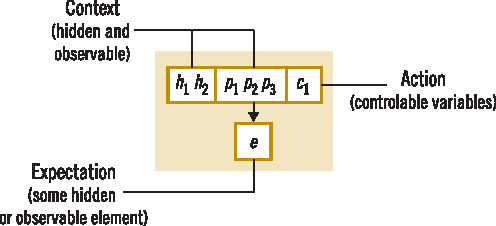
\includegraphics[width=0.6\textwidth]{Figure_4_CALM_schema.pdf}
	\caption{Perotto's schema from \cite{Perotto:2013:CF} Fig. 2.
		A schema is composed of three vectors: context containing hidden variables and observable properties $(h_1, h_2, p_1, p_2, p_3)$, action $(c_1)$, and expected result $(e)$. } 
	\label{fig:perotto_schema}
\end{figure}

The main drawback is that CALM can only identify regularities if they are deterministic, differently from the original schema mechanism, which can maintain unreliable regularities within the system in order to spinoff reliable schemas afterwards. 
To compensate that limitation, CALM introduces a new distinction between two kinds of context variables: hidden variables and observable variables as shown in the Fig. \ref{fig:perotto_schema}.
The justification is that some regularities appear as non-deterministic because the agent cannot perceive all the contextual elements necessary to precisely determine its transition function.
In this way, the accent is placed on the discovering of abstract or non-observable elements, that once introduced and integrated in the anticipatory system, are able to explain the observation, making the transition deterministic. 
The idea is, in fact, quite similar to what Dresher called synthetic items in the original mechanism, but the way to create them is slightly different: 
when an expected result is contradicted, and no elements from context or action can explain the incoherence between the prediction and the observed result, then the mechanism supposes the existence of an abstract variable that, if known, would be able do distinguish between the two situations.
The observed result then serves as a mean to deduce the value of that abstract variable, i.e. when the result corresponds to the old expectation, it is because the non-observable condition was present, and if the result is the new one, then the non-observable condition was absent, which corresponds to the state of the abstract variable perceived a posteriori.
Finally, by searching in the previous step, the mechanism can try to anticipate the contexts and actions that changes that abstract variable, like illustrated in the Figure \ref{fig:perotto_abstraction}.

\begin{figure}
	\centering
	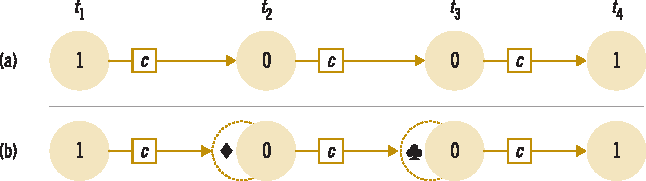
\includegraphics[width=0.7\textwidth]{Figure_5_CALM_dynamics.pdf}
	\caption{Predicting the dynamics of a non-observable property. 
	(a): An actually experienced sequence including $0 + c \rightarrow 0$ and	 $0 + c \rightarrow 1$.
    (b): The use of a synthetic element to explain the logic behind the observed transformations: $\blacklozenge 0 + c \rightarrow 0$, $\clubsuit 0 + c \rightarrow 1$, $1 + c \rightarrow \blacklozenge$,	 and $0 + c \rightarrow \clubsuit$.} 
	\label{fig:perotto_abstraction}
\end{figure}

For dealing with the combinatorial complexity, at the beginning, the only variables that CALM tries to understand and anticipate are those associated to affective values (what Drescher called primitive values).
It is like a built-in reward function that associate positive (desirable) or negative (undesirable) values that the agent can ``feel'' immediately depending on the value of the variable (i.e. its observation, e.g. true or false if boolean).
Staying focused on these variables avoids wasting energy by creating models about everything. 
Gradually, the variables needed to anticipate the evolution of some important variable (relation of causality) are then considered also important, and the mechanism will seek to model their transformation function too.

Differently from the original mechanism, which creates one initial schema for each action with empty context and result, CALM creates one initial schema for each item on the result vector (which corresponds to a perceptive variable) that has	a non neutral affective value, with empty context and action.
Each one of these initial schemas will grow up, giving rise to an anticipatory tree, responsible for identifying the relevant elements and the rules that describe the transition of its associated item, allowing in this way to anticipate it. 
Each anticipatory tree is constructed step by step using 4 operations: \textit{differentiation}, \textit{adjustment}, \textit{integration}, and \textit{abstraction}.
Each node in the anticipatory tree is identified by a vector containing observations and actions. 
Starting from a completely generic root node, where all elements on that vector are set as \textit{undefined}, the agent tries to verify if some regularity persists from the current time-step to the next.
The idea is defining a structure that is coherent with the past experience.
The expectation of that first schema will be equivalent to the first observation. 
In this way the schema tries to represent as many transitions as they can be predicted deterministically with the minimum of context (i.e. the minimum of dependencies).

When an observed result contradicts what was expected, the tree is expanded by differentiation, like illustrated in Fig. \ref{fig:perotto_diff}: the contradicted generic schema gives rise to two different children, specializing either one element of context or one element of the action vector, in order to explain the surprise, making the model coherent again.
When no primitive action or primitive context element can be used to differentiate a contradicted schema, the mechanism creates a synthetic element of context, representing some abstract or non-observable variable, that, if exists, can explain the incoherence. 
The schema is then differentiated by this new element.
Sometimes, it is not possible to differentiate the schema anymore, in this case, an adjustment is done, setting the contradicted expectation to undefined.
Finally, when several schemas are adjusted, some differentiations become unnecessary, then the tree can be pruned, and some leaf schemas integrated in a more general one.
%Another difference of CALM in relation to the original mechanism is that 
In this way, the schemas can be organized in a structure called \textit{anticipatory tree}, 
%represented in Fig. \ref{fig:perotto_tree}, 
which defines a hierarchy, like a decision tree, starting from a completely general context and action at the root node, to most specialized ones, the leaf nodes.
%
\begin{figure}
	\centering
	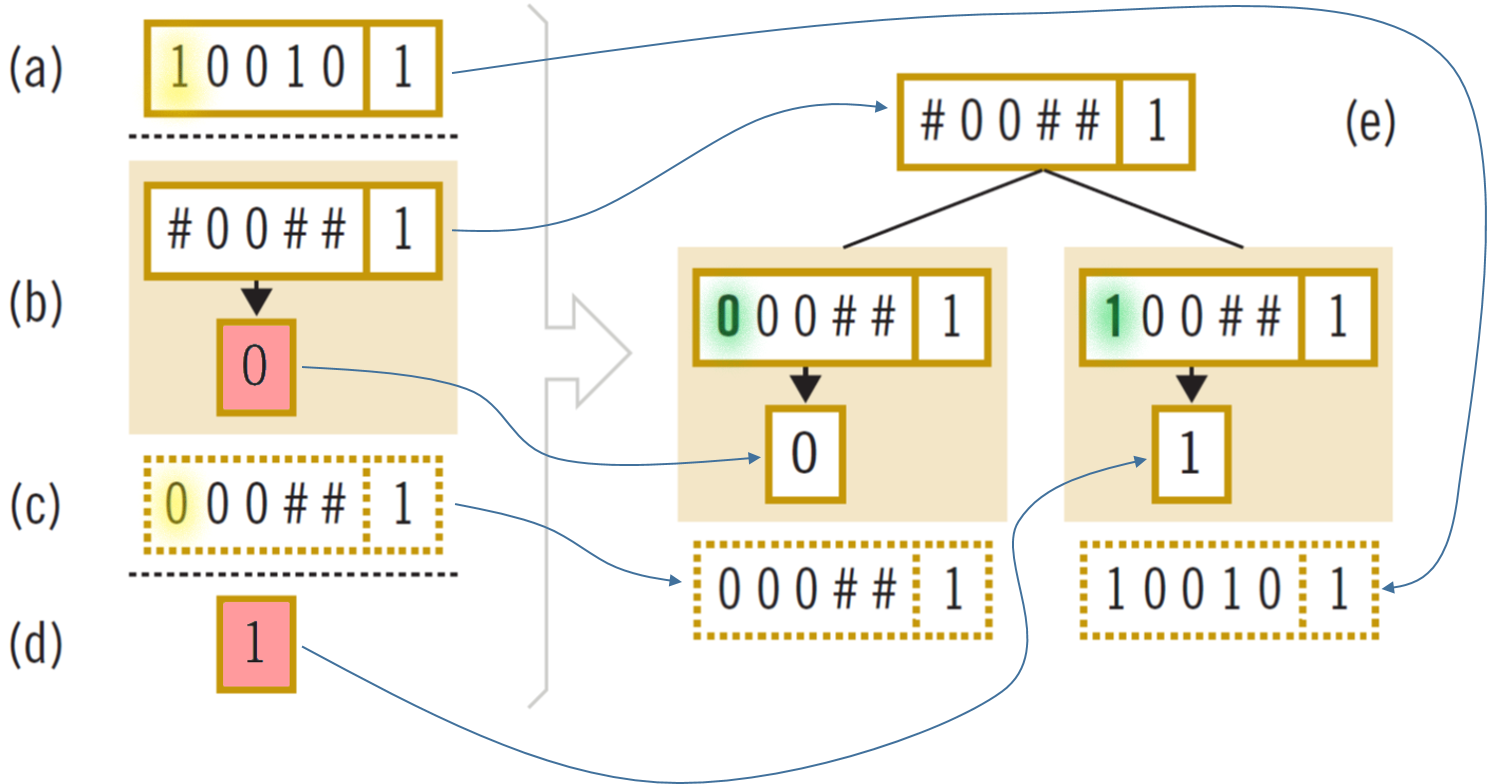
\includegraphics[width=0.6\textwidth]{Figure_perotto_differentiation_arrows.png}
	\caption{Differentiation example. 
	(a): An actually experienced situation (with five variables) and executed action (one variable). 
	(b): Activated schema (with compatible context, action, and expectation).
	(c): Associated episodic memory (representation of actual situations where the scheme has been activated, with no interdependencies between variables).
    (d): Actually observed result after the execution of the action.
    (e): Sub-tree generated by differentiation in order to compensate the divergence observed between expectation and result.} 
	\label{fig:perotto_diff}
\end{figure}

To be able to make differentiations, beyond the context and action vectors that identify the schema, the mechanism must store a kind of memory of the effective experienced contexts and actions observed during the past activations of the schema.
The identity of the schema corresponding to a maximally generic situation, and the memory corresponding to a maximally specific situation.
In order to create a new schema by differentiation, the mechanism search for an item or action in the memory of the schema that is different from the current situation that is causing the incoherence. 
The differentiation will preserve the past experience in the old schema, identifying it with a more specialized context or more precise action, separating the new situation in another schema.
In terms of computational complexity, the problem is how to manage that memory, because it needs to remember co-occurrences of items and actions.
The solution given by Perotto is to explicitly limit the number of variables to observe together, starting from 1, and gradually increasing that number, which in any case will always be low, at the order of few units.
The original mechanism proposed by Drescher faces the same problem, and is limited to observe only one additional variable at time.

Fig. \ref{fig:perotto_ben} shows the simple flip problem~\cite{Singh:2003:ICML}, used to demonstrate CALM's capability to create an abstract variable for representing a relevant non-observable condition of the environment~\cite{Perotto:2007:EpiRob}.
The set of possible actions is $\{\texttt{l},$ $\texttt{r},$ $\texttt{u}\}$, standing for \textit{go left}, \textit{go right}, and \textit{unchanged}.
The set of possible sensory signals is $\{\texttt{0}, \texttt{1}\}$, corresponding to a single primitive item in Drescher's terms.
The difficulty comes from the fact that the agent cannot directly perceive the underlying state of the world. 
The agent constructed the graph in Figure \ref{fig:perotto_tree}. 

\begin{figure}
	\centering
	%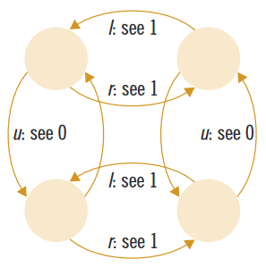
\includegraphics[width=0.3\textwidth]{Figure_perotto_benchmark.png}
	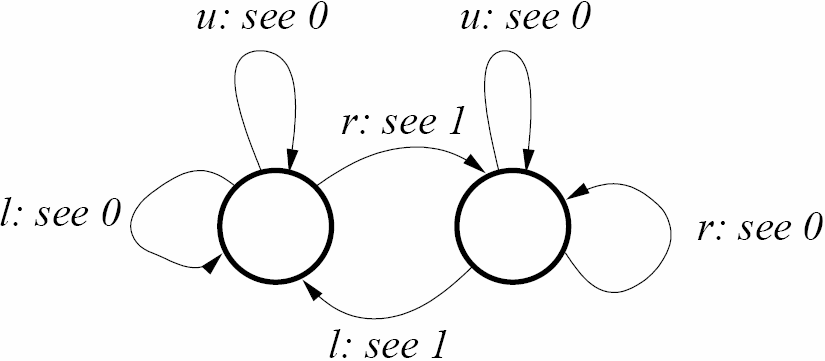
\includegraphics[width=0.55\textwidth]{Figure_flip_problem.png}
	\caption{The flip problem initially proposed by Singh et al.~\cite{Singh:2003:ICML}.
	The \texttt{r} action taken from the left states activates the right state and vice versa, yielding sensory signal \texttt{1}.
	All other cases leave the state unchanged and yield sensory signal \texttt{0}.
} 
	\label{fig:perotto_ben}
\end{figure}

In summary, CALM was used to control an agent that received only a binary sensory signal that does not directly represent the state of the environment.
This contrasts with Drescher's experiment in which primitive items represent elements of the state of the world. 
CALM is able to reconstruct \textit{non observable properties} from sequences of actions and feedback.
Similar to Drescher's synthetic items, non observable properties describe the underlying state of the world that cause this feedback. 
Another addition to Dresher's mechanism is that CALM organizes non observable properties (i.e., synthetic items) hierarchically in the anticipatory trees, which are finally mixed together, as shown in the Figure~\ref{fig:perotto_tree}, which represents the final stable solution for the %OG hyper-
flip problem.

\begin{figure}
	\centering
	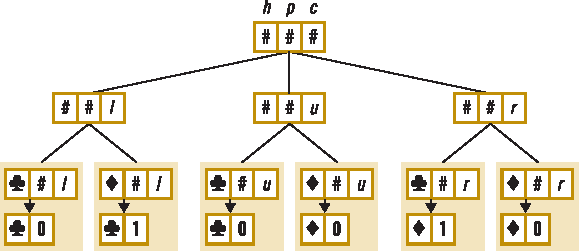
\includegraphics[width=0.7\textwidth]{Figure_8_CALM_tree.pdf}
	%\caption{Example of Perotto's anticipatory tree from \cite{Perotto:2013:CF} Fig. 10: ``Final schematic tree for solving the hyper-flip problem.''.} 
	\caption{Final schematic tree for deterministically describing the transition function corresponding to the flip problem~\cite{Perotto:2013:CF}. Note that the underlying non-observable left and right states of the problem are represented by $\blacklozenge$ and $\clubsuit$ values of the abstract sythetic variable. A \textit{Markovian Decision Process} with 4 states ($\blacklozenge 0, \blacklozenge 1, \clubsuit 0, \clubsuit 1$) and a deterministic transition function can be derived from that tree if an immediate reward function is given (e.g. $R(0) = -1, R(1) = +1$), allowing to extract an optimal policy of actions using dynamic programming techniques.} 
	\label{fig:perotto_tree}
\end{figure}

%%%%%%%%%%%%%%%%%%%%%%%%%%%%%%%%%%%%%%%%%%%%%%%%%%%%%%%%%%%%%%%%%%%%%%%%%%%%%%%%%%%%%%%%%%%%

%\subsection{Kugele's}
\subsection{Learning Intelligent Decision Agent (LIDA)}
\label{sec:lida}

The \textit{Learning Intelligent Decision Agent} (LIDA) is a broad cognitive architecture serving both as a conceptual and as a computational framework for modeling the mind~\cite{franklin_foundational_2007,franklin_2013_lida}.
A recent version of the LIDA cognitive architecture \cite{kugele_learning_2021} implements a schema mechanism inspired by Drescher on top of a perceptual memory module called the \textit{Perceptual Associative Memory} (PAM). 
Percepts are not directly received from the environment but constructed in the PAM through an active sensorimotor process. 
Other memory modules are implemented including episodic memory, declarative memory, and spatial memory.
Knowledge is represented as a directed graph called the \textit{node structure}. 

LIDA's schemas work as templates with unbound variables in their context, action, and result. 
Actions may have unbound variables that qualify and modulate how an action is executed. 
Schemas are instantiated as \textit{behaviors}. 

%FP:
LIDA implements an \textit{affective valence} 
which drives 
%The affective valence can bias 
behavior selection towards desirable outcomes. 
Liking and disliking are distinguished from wanting and dreading with the argument that they relate to distinct neural pathways in the brain \cite{kringelbach_functional_2010}. 
Wanting and dreading are qualified by \textit{incentive salience} of behaviors.   

%FP:
Kugele \cite{kugele_constructivist_2025} recently presented an improved version of LIDA into which the
%LIDA's schema mechanism to demonstrate contstructivist learning.
primitive items are replaced by \textit{amodal nodes} organized in the node structure in Perceptual Associative Memory. 
An important difference between LIDA's amodal nodes and Drescher's primitive items is that amodal nodes may not only represent sensory data but also events. 
Consequently, LIDA can not only represent a particular context in terms of elements of the world state, but also in terms of sensorimotor events. 

Fig. \ref{fig:lida} shows the cognitive cycle. 
The dashed rounded rectangle at the bottom shows the schema mechanism as a part of the architecture. 
The Global Workspace (right) stores a description of the current situation as a graph node. 
The Procedural Memory module (bottom right) is the memory of schemas. 
The graph node from Global Workspace activates relevant schemas. 
The Action Selection module selects an action, primitive or composite, from among the actions of the relevant schemas. 
Once the action is selected, it is instantiated as a \textit{behavior}, or a \textit{stream of behavior} for composite actions, and their unbound variables are qualified. 
The behavior is enacted in the Environment (left) and sensory stimuli (signals) are received by the Sensory Memory module (upper left).
Sensory signals are processed to produce amodal nodes that represent the current situation. 
The Attention Codled module selects some amodal nodes to broadcast in the Global Workspace module. 

\begin{figure}
	\centering
	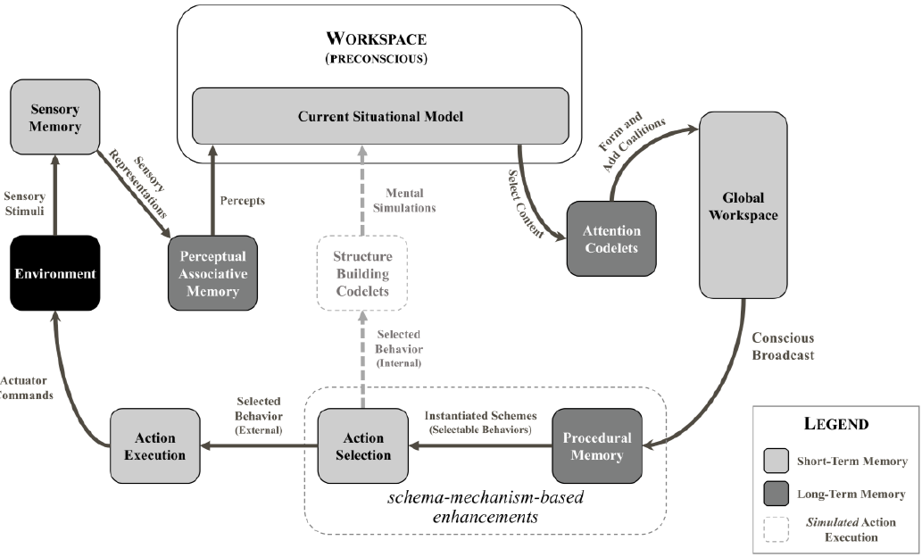
\includegraphics[width=0.7\textwidth]{Figure_LIDA.png}
	\caption{Simplified depiction of the LIDA cognitive cycle \cite[Fig. 4]{kugele_constructivist_2025}.
	} 
	\label{fig:lida}
\end{figure}

Kugele \cite{kugele_constructivist_2025} demonstrated constructivist procedural learning within LIDA in a multi-armed bandit environment.
Different versions of k-armed-bandit environments have been used previously, for example to demonstrate the theory of \textit{active inference} \cite{smith_step-by-step_2022}, 
but Kugele added new difficulties by requiring the agent to sit and to make a deposit before playing.  
When the agent is standing (State $S$), it can take the action to sit at a one-armed bandit machine, for example Machine 1 (State $M_1$).
The agent can then pay a deposit (state $M_1P$), and then play, which may yield a win (State $M_1W$) with probability $p(W|M_1P)$, or a loss (State $M_1L$) with probability $p(L|M_1P)$. The agent can choose to stand from any state.
Fig. \ref{fig:lida_bench} represents the state diagram of this environment in the case of two machines. 

\begin{figure}
	\centering
	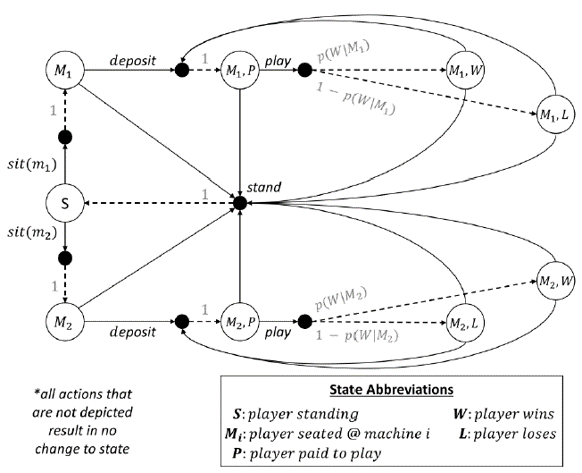
\includegraphics[width=0.7\textwidth]{Figure_LIDA_bench.png}
	\caption{State diagram of the 2-armed bandit environment \cite[Fig. 5]{kugele_constructivist_2025}.
	White nodes depict environmental states.
	Black nodes depict actions. 
	Links going from white state nodes into black action nodes indicate that this action is taken from that state. 
	Dashed links leaving action nodes are labeled with the probabilities of transitioning to possible states resulting from this action.} 
	\label{fig:lida_bench}
\end{figure}

The set of possible actions for k machines is $\{ \texttt{stand}, \texttt{sitM1},..., \texttt{sitMk},$ $\texttt{deposit},$ $\texttt{play} \}$. 
The set of initial nodes is $\{\texttt{Win}, \texttt{Lose} \}$, corresponding to a single primitive item in Drescher's terms.
Node \texttt{Win} is associated with the affective valence (i.e., primitive value) of $+1$, and Node \texttt{Lose} of $-1$.   
As in the flip problem presented above, the agent cannot directly perceive the state of the environment.
The results obtained in an 8-armed-bandit environment show that after 25,000 interaction cycles, the agent successfully constructed the amodal nodes (i.e., synthetic items) $\{ \texttt{S}, \texttt{M1},  ..., \texttt{M8}, \texttt{M1P}, ...,  \texttt{M8P} \}$ that represent the states of standing or sitting at a machine without or with a paid deposit, along with the schemas representing the transition between states. 
Once this was learned, the agent determined and chose the machine that yielded the highest payoff.

In summary, LIDA allowed an agent that receives only a binary sensory signal (\texttt{Win} or \texttt{Lose}) to learn the structure of this environment, and to find adapted behaviors (sitting at the most favorable machine, and then continuing to deposit and to play) satisfying the motivation of maximizing the value won. 
This is similar to CALM but in a more complex environment.

The agent's adaptation to the k-armed bandit environment was made possible by LIDA's distinction between sensory signal and perceptual memory that allows treating sensory signal as mere events rather than elements of the state. 
Notably, the agent did not learn the states \texttt{MiW} and \texttt{MiL} but rather the aggregated state $\texttt{Mi}$ representing sitting at Machine $i$.
This is because the sensory item (\texttt{W} or \texttt{L}) is not useful in itself to differentiate significant states from the agent's viewpoint. 
%Instead, they are mere feedback from the \texttt{play} action. 
%This stands in contrast from Drescher's assumptions that use primitive items as elements of the states. 

Another difference is that LIDA treats composite schemas as procedural knowledge (stream of behavior) that are handled as a whole action by the Action Execution module, which facilitates the learning of the sequence \texttt{deposit}--\texttt{play}, before finding the machine that yields the highest payoff. 

%%%%%%%%%%%%%%%%%%%%%%%%%%%%%%%%%%%%%%%%%%%%%%%%%%%%%%%%%%%%%%%%%%%%%%%%%%%%%%%%%%%%%%%%%%%%

%\subsection{Georgeon's}
\subsection{Enactive Cognitive Architecture (ECA)}

Olivier Georgeon and colleagues also studied problems in which the agent receives little sensory information and must find behaviors that satisfy its predefined motivational criteria \cite{georgeon_intrinsically-motivated_2012} . 
Similar to CALM and LIDA, Georgeon's schemas are based on events of interaction that do not necessarily represent elements of relevant states.  

Formally, schemas are tuples $\langle$pre-subschema, decision, post-subschema$\rangle$ in which the pre-subschema and the post-subschema are other schemas.  
The mechanism is initialized with a set of \textit{primitive schemas} that define the primitive possibilities of interaction of the agent with its environment. 
Primitive schemas are initialized with a predefined valence (equivalent to Drescher's primitive value and LIDA's affective valence) that specify the agent's ``inborn'' preferences of interaction. 

In the case of a simulated agent, a primitive schema is the association of a \textit{primitive action}, for example \texttt{move-forward} or \texttt{turn}, with a \textit{primitive outcome}, for example \texttt{bump} or \texttt{no-bump}.  
The primitive schema $\langle$\texttt{move-forward}, \texttt{bump}$\rangle$ initialized with a negative valence specifies an agent that ``dislikes'' bumping into walls when it tries to move forward. 

%In contrast with Drescher's and Perotto's mechanisms, however, pre-conditions and post-conditions are not properties of the world (hidden or observed) but are other schemas learned previously. 
The mechanism learns new schemas from the bottom up, with higher-level schemas made of a sequence of two previously-learned subschemas, 
as illustrated in Fig. \ref{fig:agent8}. 
Schemas are noted with the letter $i$ because they are sometimes called \textit{interactions}.
For example, if the primitive schema $i00$, made of action $a0$ and outcome $o0$, was enacted at time $t-2$, and the primitive schema $i11$, made of action $a1$ and outcome $o1$,  was enacted at time $t-1$, then the composite schema $\langle i00, a1, i11 \rangle$ is learned (added to memory) or its \textit{weight} is incremented if it already existed. 
The weight of schemas plays a similar role as their reliability in Drescher's implementation.

When a new schema's post-subschema is primitive, the new schema's decision consists of performing the post-subschema's action.
When the post-subschema is composite, the new schema's decision consists of enacting the whole sequence specified by the post-subschema. 
This mechanism constructs a hierarchy of schemas similar to LIDA's hierarchical streams of behaviors. 

At time $t$, the previously learned schemas whose pre-subschemas match the current situation are \textit{activated}.
Activated schemas compete to propose their decisions according to a \textit{proclivity value} computed from the activated schema's weight and the post-subschema's valence. 

A decision to enact a composite schema generates a stream of behavior consisting of sequentially enacting the whole sequence of primitive schemas that constitute this composite schema.  
If the enaction of any of its primitive subschemas fails (i.e., the actual outcome differs from the schema's outcome), then the enaction of the sequence is interrupted. 

%The mechanism is not initialized with a top-level goal. 
%Instead, it is initialized with a predefined set of low-level primitive schemas that define the agent's basic possibilities of interaction. 

\begin{figure}
	\centering
	\includegraphics[width=1.0\textwidth]{Figure_3_agent8.pdf}
	\caption{Schema learning and selection.
		Schemas are nested tuples: $\langle$pre-subschema, decision, post-subschema$\rangle$.
		Over time, new decisions and new schemas are learned from the bottom up. 
		Recently enacted schemas (in gray) activate the previously-learned higher-level schema whose pre-subschema they match.
		Activated schemas propose their post-subschemas with a proclivity value calculated from the activation weight and the expected valence.
		The schema with the highest proclivity is selected to try to enact.} 
	\label{fig:agent8}
\end{figure}

%The schema learning mechanism and selection works as follows.
%At the end of time step $t$, the agent records or reinforces the schemas: 
%\begin{itemize}
%	\item[$\bullet$] $(i_{t-2}, d_{t-1}, i_{t-1})$
%	\item[$\bullet$] $((i_{t-3}, d_{t-2}, i_{t-2}), d_{t-1}, i_{t-1})$
%	\item[$\bullet$] $(i_{t-3}, d^2, (i_{t-2}, d_{t-1}, i_{t-1}))$
%	\item[$\bullet$] $((i_{t-4}, d_{t-3}, i_{t-3}), d^2, (i_{t-2}, d_{t-1}, i_{t-1}))$
%\end{itemize}

%If it does not yet exist, the new decision $d^2$ is constructed different from the decision $d_{t-2}$ that was actually made at time $t-2$. 
%For example, if the agent made decision $d_{t-2} = a0$ and enacted interaction $i_{t-2}=i00$, and then made decision $d_{t-1} = a0$, and enacted interaction $i_{t-1}=i01$, the agent learns the new decision $d^2=i00a0$ consisting of trying to enact the interaction $i_t=i00$ and then do action $a_{t+1}=a0$. 
%When decision $d^2$ has been selected and successfully enacted, the mechanism learns higher-level schemas on top of it. 
%The rate of schema construction being constant, the number of schemas grows linearly with time. 
%Older and unused schemas can be forgotten.

Georgeon \cite{georgeon_small_2012} reports an experiment in the environment shown in Fig. \ref{fig:georgeon} and shared in a video \cite{georgeon_video_2012}.
The set of primitive actions is $\{ \texttt{move-forward},$ $\texttt{turn-left},$ $\texttt{turn-right},$ $\texttt{feel-front},$ $\texttt{feel-left},$ $\texttt{feel-right}\}$.
The set of possible outcomes is $\{ \texttt{no-wall},$ $ \texttt{wall} \}$ corresponding to a single primitive item. 
%The \texttt{turn} actions always yield the \texttt{no-wall} outcome.
The schema $\langle$\texttt{move-forward}, \texttt{no-wall}$\rangle$ has a valence of $+5$ making it the only ``enjoyable'' interaction to the agent. 
The schema $\langle$\texttt{move-forward}, \texttt{wall}$\rangle$, corresponding to bumping into wall, has a valence of $-10$ making it strongly dreaded. 
The 6 schemas that have a \texttt{feel} action have a valence of $-1$ making them slightly costly. 
The schemas that have a \texttt{turn} action  have a valence of $-3$ making them mildly costly. 

Like in the experiments with CALM and LIDA presented above, the difficulty comes from the fact that the agent only has a single binary sensory signal and cannot directly sense the state of the environment. 
The agent thus characterizes the state of the environment through enacted schemas. 
Results show that after approximately a hundred interaction cycles, the agent learns to use the \texttt{feel} schemas to actively sense the environment. 
This active sensing provides a situation awareness that makes the agent turn to empty cells when necessary, avoid bumping into walls, and optimize its moving forward. 

\begin{figure}
	\centering
	
\includegraphics[width=0.3\textwidth]{Figure_grid_plot.pdf}
	\caption{The small loop Challenge \cite{georgeon_small_2012}.
		The agent can move forward to an empty (white) cell, bump into a wall (green cell), turn to the left or to the right by 90°, or ``feel'' the cell in front, to the left, or to the right. 
		The sensory signal is a single-bit feedback from the action (``empty'' or ``wall''). 	
		The agent progressively learns to used the ``feel'' schemas to sense its surrounding environment, not move forward when it feels a wall in front, and turn to a direction where it feels no wall, thus maximizing the ``move forward'' interaction that has a predefined positive valence.
	} 
	\label{fig:georgeon}
\end{figure}

In a robot, primitive actions are defined as hard-coded control loops that regulate actuators and monitor sensory feedback over a predetermined period. 
For example, the \texttt{move-forward} action turns on the wheel engines and runs a loop that monitors the elapsed time and the collision detection sensor. 
If a collision is detected, the schema is terminated before its predetermined duration. 
Upon termination, the wheel engines are turned off and the outcome is sent to the schema mechanism, for example \texttt{no-bump} or \texttt{bump}.

To deal with the complexity of the physical world, Georgeon and colleagues encapsulated the schema mechanism in a cognitive architecture called Enactive Cognitive Architecture (ECA) \cite{georgeon_eca_2013}.
ECA incorporates a spatial memory module that can simulate the enaction of schemas to help select the most desirable schema in the current spato-temporal context. 
Like in LIDA, schemas may include unbound variables that can be qualified upon their instantiation. 
For example, the \texttt{turn} action has the variable \texttt{angle} that specifies the rotation span in the horizontal plane (yaw).
When the schema mechanism module selects the \texttt{turn} action, the spatial memory module qualifies the angle to the desired direction.

%Georgeon \cite{georgeon_artificial_2024} demonstrated 
ECA was demonstrated with the robot shown in Fig. \ref{fig:robot} \cite{georgeon_artificial_2024}.
When the robot finds reliable schemas in a consistent spatial localization, it creates a datastructure called a \textit{phenomenon} that represents the ``thing'' in the world that affords these schema.
This is analogous to the construction of synthetic items in Drescher's schema mechanism.

\begin{figure}[htbp]
	\centering
	\begin{subfigure}{0.49\textwidth}
		\centering
		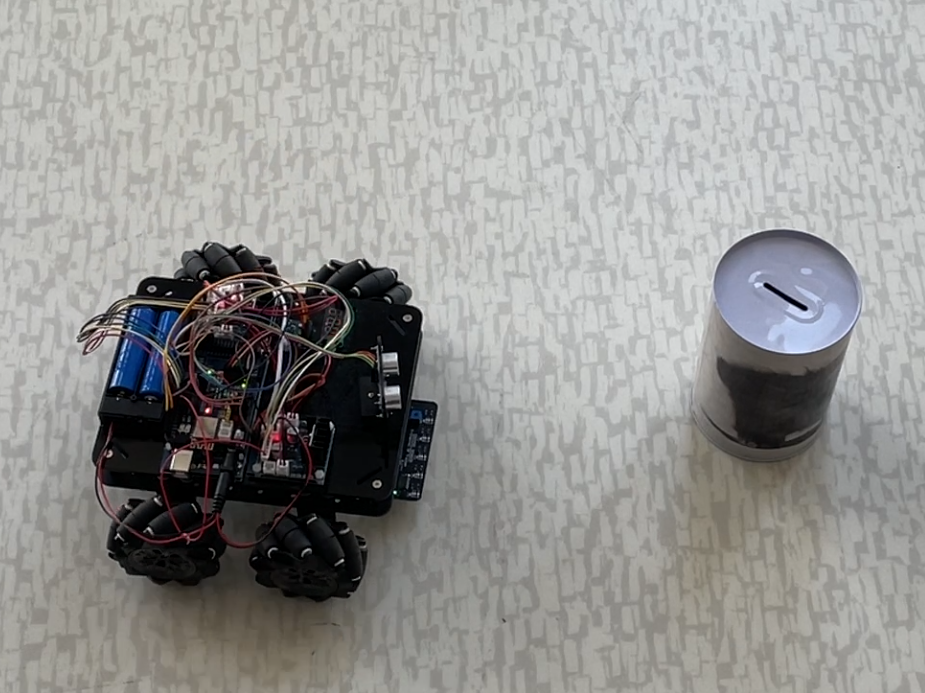
\includegraphics[width=\linewidth]{Figure_petitcat.png}
		\label{fig:first}
	\end{subfigure}
	\hfill
	\begin{subfigure}{0.49\textwidth}
		\centering
		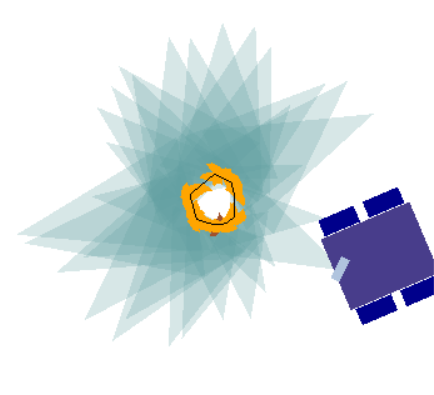
\includegraphics[width=\linewidth]{Figure_phenomenon.png}
		\label{fig:second}
	\end{subfigure}
	\caption{Robot learning a phenomenon (synthetic item) representing a cylindrical object \cite[Fig. 5]{pmlr-v192-georgeon22a}.
		Left: Photo of the robot showing its ultrasonic echo-localization sensor mounted on its pivoting head. 
		Right: Representation of the \textit{cylindrical phenomenon}.
		The phenomenon is aggregated from many sensorimotor ``manifestations'' of the cylindrical object through echo-localization measures. 
		Blue triangles represent the cones of the ultrasonic signals sent by the robot over time from different positions around the moneybox.
		The black line is the shape of the cylindrical object reconstructed from the echoes. 
	}
	\label{fig:robot}
\end{figure}


In summary, ECA's schema mechanism uses schemas as atomic elements for constructing higher-level schemas instead of sensory signals, synthetic items, and actions.
This design choice facilitates the hierarchical leaning of composite schemas because they are not based on abstract representations of elements in the world.
In the experiment reported in Fig. \ref{fig:georgeon}, the agent manages to adapt to its environment using only schemas but no synthetic items.
Like Drescher and Kugele, Georgeon implemented an effect of \textit{habituation} that causes reliable schemas to be preferably reused, which facilitates the construction of higher-level schemas on top of them. 
This habituation principles has echoes in Woolford's \textit{sensorimotor sequence reiterator} \cite{woolford_precarious_2020}.
%The learning process is funneled by ``innate'' preferences of interaction. 


ECA makes a strong design choice by assuming that the environment has a three-dimensional Euclidean structure and is populated with physical objects. 
This assumption is coded in the cognitive architecture through the spatial memory module and by adding unbound variables to schema that encode spatial parameters. 
This design choice allows ECA to construct phenomena to represent ``things'' in the physical world. 
We hypothesize that it can help avoid the scalability limitation of Drescher's implementation of synthetic items. 
Including spatial variable in schemas and qualifying them adequately, however, raises many questions that remain open. 

%learns habits of interaction that are organized hierarchically, with shorter sequential habits learned first, and longer sequences of habits made of sequences of shorter habits later learned on top of them. 

%%%%%%%%%%%%%%%%%%%%%%%%%%%%%%%%%%%%%%%%%%%%%%%%%%%%%%%%%%%%%%%%%%%%%%%%%%%%%%%%%%%%%%%%%%%%

%\subsection{Thorisson's}
\subsection{Autocatalytic Endogenous Reflective Architecture (AERA)}

%AERA\footnote{Autocatalytic Endogenous Reflective Architecture; see www.openaera.org – accessed Dec. 6th, 2024.} is a unified system that can learn about causal relations cumulatively, from experience \cite{thorisson2019cumulative,thorisson2014autonomous,nivel2013autocatalytic}. The system’s knowledge representation uniquely combines ampliative reasoning, autonomous resource management, explanation-driven compositional knowledge representation and reflection in a synergetic architecture that can grow its knowledge from a small “bootstrapping seed” \cite{thorisson2020seed}. Its compositional knowledge contains numerous peewee-size “micro-models” that can be combined in explainable ways to model experience \cite{thorisson2021explanation}. 

%The methodology behind AERA rests on three fundamental principles \cite{thorisson_seed-programmed_2020,thorisson2012new,nivel2009self}: 1. During learning, a learner autonomously creates new knowledge through a variety of methods including hypothesis generation and testing; 2. autonomous learning must create models of causal relations through situated goal-driven reasoning, and 3. self-programming is based on transparent operational semantics based on peewee-size uniform knowledge models. 
%Those familiar with Piaget’s \cite{berlyne2003psychology} fundamental insight that human learning requires creation of new information will recognize the first principle. 
%For this principle, Piaget proposed the idea of schemas – information structures that mediate between perception and action, capturing and controlling experience. 
%An important difference between AERA’s knowledge representation and other schema mechanisms
%proposals based on this idea (cf. \cite{arbib2003handbook,drescher_made-up_1991}) 
%is its emphasis on non-axiomatic worlds and the resulting strong requirement for transversal defeasibility of acquired knowledge (cf. \cite{pollock1987defeasible}) – in other words, that since no certainty about anything learned can be guaranteed, the methods for knowledge creation cannot be based on the assumption of knowledge of a “ground truth”. The methodology behind AERA unifies this, and the above listed assumptions, in a coherent theoretical approach, with deep implications for knowledge creation in light of novelty: AERA starts out with only a tiny amount of “bootstrap” (seed) knowledge – the remainder of its knowledge, which soon vastly outsizes the seed\footnote{In our implementation of S1 – an AERA agent that learns to do TV-style interviews, the ratio of the learned knowledge over the seed knowledge, after 20 hours of learning, was ~53 \cite{thorisson2014autonomous}.}, is then generated autonomously by the system itself, based on hypotheses that are inspired and verified through experience, using ampliative reasoning mechanisms. 

%\begin{itemize}
%	\item The knowledge representation in AERA is peewee (relatively small) and compositional; AERA can inspect, deconstruct, and reconstruct its models, as well as create hierarchies of models of its experience.
%	\item The models in AERA are falsifiable, have degrees of confidence, and can be related to specific groups with certain attributes specifying their context.
%	\item The choice of models and reasoning methods at any point in time is dynamic, based among other things on the extent of available resources (models and time).
	
%\end{itemize}

AERA’s models \cite{thorisson2019cumulative,thorisson2014autonomous,nivel2013autocatalytic}, similar to Drescher’s schemas \cite{drescher_made-up_1991} and the neuro-symbolic approach presented in \cite{komrusch_symbolic_2022}, represent knowledge by contextualized programs that capture antecedental and successional states of important relationships (e.g. the relationship between a hand and an object that one wants to pick up). 
Unlike these, AERA places explicit representation of cause-effect relations at its core \cite{thorisson2018cumulative}. 
During its continuous learning, driven by a self-maintained dynamic goal hierarchy, the most useful (effective and efficient) models of cause-effect relations encountered in the environment are retained, while others are discarded. 
Based on predictions, informed experimentation, and strategic induction, the system autonomously creates new knowledge cumulatively, effortlessly unifying new information with old, even in light of contradictions. Further separating AERA from other approaches are its atomic elements for knowledge creation, whose operational semantics are transparent to the system’s own reasoning, meaning that they can be inspected and learned by the same explicit, defeasible unified reasoning mechanisms as used for learning about the world. 

%The approach uniquely unifies cognition and meta-cognition in a single, coherent architecture, enabling efficient and effective self-reflection that lays a foundation for a capacity for cognitive growth. The result is a system that can dynamically employ ampliative reasoning, at any point in time, to predict both the immediate and far future, including its own cognitive resource use (“think time”). 

Key representational components of this approach include \cite{sheikhlar2024autonomous,sheikhlar2024causal}: 
\begin{itemize}
	\item \textbf{Facts} are statements that represent a cognitive event, e.g. operations happening in AERA itself; facts are the only entity in AERA that have complete certainty (corresponding to Descartes' axiom “I think, therefore I am”).
	\item A \textbf{composite State model (CST)} captures a set of simultaneous (timeless) Facts that the AERA system considers to be (potentially) useful and/or necessary for properly predicting an event’s consequences; used to e.g. represent a variety of subsets in the world such as spatial relations of objects, the values of a perceived object’s properties, such as its position and color, etc. %The forming of a CST at time T becomes a Fact with a timestamp T and a GUID (i.e. it is certain to the AERA executive that this CST was formed at time T). 
	\item A \textbf{cognitive event model (CEM)} captures a (hypothesized) causal influence of a Fact on another Fact; used to represent the effect that an action or event in particular circumstances, e.g. a command initiated by AERA at some timestep, has on the state of the world at a later timestep. When a CEM fires it produces a prediction (while the production of a prediction is represented as a Fact, the confidence in the prediction itself is defeasible and is in part based on the confidence of the CEM).
	\item A \textbf{requirement model ($M_{req}$)} captures the (predicted) requirements/\hspace{0pt}conditions that must be met for a CEM to be relevant in a particular context at a particular time.
%	
\end{itemize}

AERA’s programming paradigm allows the system itself to inspect these types of information structures, use them “for parts” to create variations, as well as create new ones from scratch. AERA’s programming language, Replicode, allows it to autonomously use these building blocks for self-programming, in the form of coherent plans, predictions, and goals that it can pursue \cite{nivel2013towards,nivel2013replicode,thorisson2012new}. 

Both \textit{CEM}s and $M_{req}$s have a left-hand side (LHS) and a right-hand side (RHS), composed of sets of Facts and constraints (e.g., math equations). The LHS Facts describe (assumed) conditions under which the RHS Facts would be produced. Figure \ref{fig:AERA} shows how the above components lead to making a prediction. When some sensory Facts match everything in a \textit{CEM}’s LHS, a relevant $M_{req}$ allows the \textit{CTS}’s instantiation, which means the conditions for making a prediction via a \textit{CEM} are met. A successful instantiation of a \textit{CEM} means that everything in its RHS will happen. 
% (probably – because all knowledge in AERA is defeasible) PR and OG. 
As the \textit{CEM} predicts a future state after an event’s occurrence, this is verified and marked as a “successful prediction” by AERA only if the prediction matches the state that is observed.

\begin{figure}
	\centering
	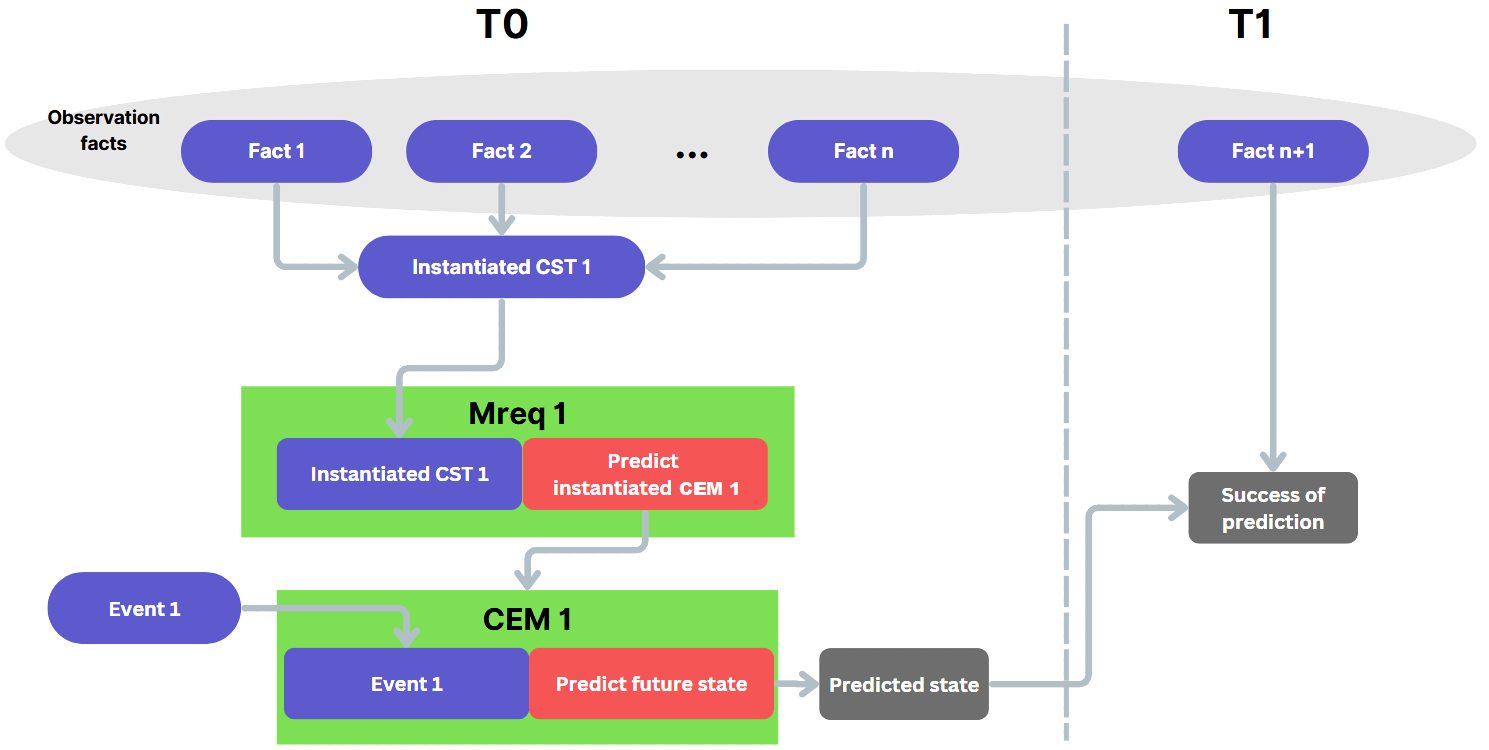
\includegraphics[width=0.99\textwidth]{AERAblockdiagram2.png}
	\caption{The connection between $CST$, $M_{req}$, and $CEM$. 
		Time T0 (left): The observation facts matching $CST1$ allow $M_{req}$ to trigger a prediction by instantiating $CEM1$. 
		Time T1 (right): AERA checks whether the observations match the predicted state.} 
	\label{fig:AERA}
\end{figure}

As an example, the triad of $CST1$, $M_{req}1$, and $CEM1$ can represent the physical movement behavior of an entity when it collides with another entity (e.g., a hand). $CEM1$ represents the dynamics of the movement, connecting the collision event (left-hand side of $CEM1$) to the moved entity’s new position (right-hand side of $CEM1$). $CST1$ represents the preconditions of the behavior, such as the entities’ position, weight, etc., and the fact that the point of collision and the moved entities' position must initially be the same. $M_{req}1$ predicts that if a striking entity hits another entity with the conditions described by $CST1$, the stricken entity’s position will change a specific amount in the next time step.

The interactions of the operational principles of AERA are quite intricate in their entirety; important aspects that are covered elsewhere include induction – the creation of new knowledge – unified abduction-deduction – the creation of plans and explanations – and runtime relevance computations \cite{nivel2013towards}. The unified integration of these operational principles in a single coherent architecture is what gives AERA its power, allowing its seed – initial human-provided knowledge – to be orders of magnitude smaller than what AERA can create on its own through learning from experience. 

These mechanisms have been demonstrated for control of virtual robots, learning and using language, and multimodal interaction \cite{thorisson2014autonomous}.
Fig. \ref{fig:robot_aera} shows the latest experiment reported in \cite{sheikhlar2024autonomous} and shared in video  \cite{Sheikhlar_video_2024}. 
The task has a \textit{guided experimentation} phase, during which the experimenter tele-operates the robot, and a \textit{task solving} phase, during which the robot must autonomously learn to grasp new objects it has never grasped before, which are novel in shape but familiar in size.
%The robot learns that the size of objects is significant in determining the correct way of grasping them.

During the guided phase, commands and successful grasping events makes AERA learn triads of Causal Event Models (CEMs), Composite State models (CSTs), and requirement models (Mreqs) for each command. 
During the task-solving phase, the analogy process induces new grasping models based on the objects’ familiarity.
Results show that, after several trials unsuccessfully testing the learned models, AERA induces new CSTs and Mreqs capable of triggering the appropriate actions. 

\begin{figure}
	\centering
	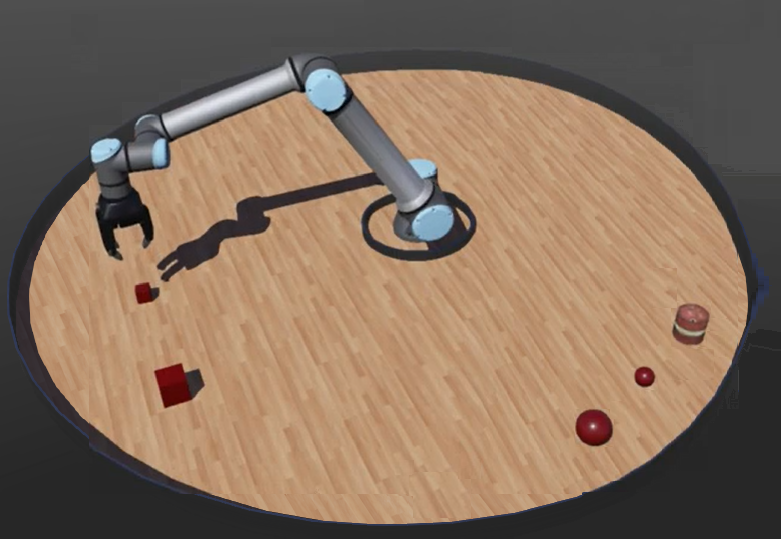
\includegraphics[width=0.5\textwidth]{Figure_Robot_AERA.png}
	\caption{Experimentation from \cite[Fig. 2]{thorisson_causal_2024}.
	In the guided phase, the robot is tele-operated to grab the small and big cubes on the left; 
	in the task solving phase, it quickly learns to autonomously grab the small ball, big ball, and big cylinder on the right by analogy.} 
	\label{fig:robot_aera}
\end{figure}

In summary, AERA introduces the capacity for the schema mechanism to process events that have en external cause in addition to those caused by the actions initiated by the agent.
This is done by distinguishing the context in which the event occurs, represented by Composite State models (CSTs), from the hypothetical causal effects of the event stored in Cognitive Event Models (CEMs).
The agent can thus construct hypothetical causal models as it passively observes other agents interacting with the world %(including other agents),
 or as it observes its own interactions while being tele-operated.
The agent can then test the hypothetical causal models by itself to evaluate their reliability. 

Both the events caused by the agent's actions and those passively observed generate the instantiation of cognitive events and the generation of \textit{prediction facts}.  
%Prediction facts are later compared with actual facts to assess the reliability of the CEM.
AERA considers both external events and cognitive events as actual facts that AERA can internally process, which opens the way to reflexivity. 


%%%%%%%%%%%%%%%%%%%%%%%%%%%%%%%%%%%%%%%%%%%%%%%%%%%%%%%%%%%%%%%%%%%%%%%%%%%%%%%%%%%%%%%%%%

\section{Conclusion}

Schema mechanisms are characterized by their dynamic approach to constructing concepts from experience of interaction.
Compared to more classical techniques such as statistical symbol grounding \cite{harnad_symbol_1990} or active inference \cite{friston_active_2017}, this dynamic approach takes into account counterfactual sequences of interactions for the construction of concepts. 
This makes schema mechanisms particularly reflect Piaget's core idea that sensorimotor schemas serve as the initial instruments for constructing knowledge. 

The four new schema mecanisms presented here, CALM, LIDA, ECA, and AERA, bring an additional  idea to the picture: the capacity to deal with sensory signals (primitive items) that are not ``percepts representing elements of the world'', but mere feedback from action or events of interaction.  
In so doing, these four new schema mechanisms address a limitation pointed out by Bettoni when he wrote that 
``Drescher's constructivism is not Piaget's constructivism, mainly because of its tacit acceptance of cognitive dogmatism'' \cite[p. 6]{bettoni_made-up_1993}.
We interpret this critique as suggesting that using primitive items that represent elements of the state falls within cognitive dogmatism because it implements the assumption that the agent has direct access to the ontology of the world.
In contrast, constructing schemas from interactional events better reflects Piaget's idea that knowledge arises from an
initial ``complete un-differentiation between the subject and the object''. 

%U  in which  sensory ``patterns and structures of objects, attributes, relations, etc. [...] be as much as possible true copies of `original' objects, attributes, relations etc. in the world'' \cite[p. 1]{bettoni_made-up_1993}.

Basing schemas on interactional events is particularly important when designing the agent's control system. 
Drescher's agents sought goal states defined in the environment---a form of \textit{extrinsic motivation} 
that is inherently prone to scalability issues as the complexity of the environment grows.
In contrast, the new schema mechanisms seek rewarding interactions as illustrated in the experiments above: CALM: moving left and right, LIDA: winning, ECA: moving forward, and AERA: grabbing objects. 
This is a form of \textit{interactional motivation} \cite{georgeon_interactional_2012} whose complexity may not grow as the complexity of the environment grows, allowing easier transfer to robots in the open world.

LIDA and ECA have demonstrated interactional motivation using both negatively valenced primitive schemas (e.g., LIDA: \texttt{deposit}, ECA: \texttt{feel} and \texttt{turn}) and positively valenced ones (LIDA: \texttt{win}, ECA: \texttt{move-forward}).
They learn composite actions made of sequences of both kinds of schemas (LIDA: $\langle$\texttt{deposit}, \texttt{win}$\rangle$, ECA: $\langle$\texttt{turn}, \texttt{move-forward}$\rangle$), which allows the emergence of behaviors adapted to delayed reward.
%This is made possible by the fact that both systems can enact sequences as a whole. 
These sequences work as short programs that the agent can re-execute,  which leads to self-programming---an important aspect of constructivist epistemology \cite{georgeon_cash_2019}.

CALM has focused on the construction of hierarchies of synthetic items, exploring Piaget's idea of assimilation and accommodation. 
%AREA has focused on international simulation, which facilitates the qualification of unbound variables of actions during the instantiation of behavior. 
LIDA, ECA, and AERA have encapsulated the schema mechanism within a cognitive architecture. 
They handle schemas with unbound variables, reducing the number of schemas and helping manage complexity, albeit at the cost of potentially diminishing generality. 
These cognitive architectures internally simulate the enaction of the schemas before selection and qualification. 
AERA has further explored this direction by allowing reflexivity upon internal events. 
Altogether, the four new schema mechanisms extend our vision of how Piaget's ideas can be translated into artificial intelligence. 
Because they incorporate significantly more of constructivist epistemology than Drescher's original version, we propose to call them schema mechanisms 2.0. 
Fig. \ref{fig:venn} synthesizes their contributions. 


\begin{figure}
	\centering
	\includegraphics[width=0.8\textwidth]{Figure_venn.pdf}
	\caption{Coverage of principal dimensions by schema mechanisms 2.0.} 
	\label{fig:venn}
\end{figure}

Schema Mechanisms 2.0 have still not passed the sensorimotor stage of development\hspace{0pt}---the first defined by Piaget. 
The question whether their implementation in computers is overly reductionist compared to biological systems remains open.
They nonetheless demonstrate some promising results with robots. 
LIDA and ECA have implemented an Euclidean spatial memory module and an intuitive physics engine to handle schemas that encode physical properties. 
This is a strong commitment that reduces generality but may open the way to developmental artificial intelligence for autonomous robots in the open world. 



%Table \ref{tab:comp} shows a comparison by the schema mechanisms presented in this paper.

%\begin{table}
%	\centering
%	\caption{Comparison of schema mechanisms}\label{tab:comp}
%	\begin{tabular}{|l|c|c|c|c|c|}
%		\hline
		%&  Drescher & Perotto & AERA & LIDA & ECA \\
%		&  MARCSYST & CALM & AERA & LIDA & ECA \\
%		\hline
%		Explicit goal & \checkmark & \checkmark & \checkmark & \checkmark &  \\
%		Concept invention & \checkmark & \checkmark &  &  &  \\
		%Marginal attribution & \checkmark & \checkmark & \checkmark & \checkmark & \\
		%Hierarchical goals &  & \checkmark & \checkmark &  &  \\
%		Non-representational sensory signal &  &  &  & \checkmark & \checkmark \\
%		Intrinsic motivation &    &  &  & \checkmark & \checkmark \\
		%Sequential schemas &    &  &  & \checkmark & \checkmark \\
		% Active perception &    &  &  &  & \checkmark \\
%		3D spatial schemas &    &  &  & \checkmark & \checkmark \\
		% Reflexivity &    &  & \checkmark & \checkmark &  \\
		% Defeasibility of acquired knowledge &    &  & \checkmark &  &  \\
%		Self-programming &    &  & &  & \checkmark \\
%		\hline
%	\end{tabular}
%\end{table}




%Indeed, theories of enaction as well as of radical constructivism have insisted that we should not take the sensory signals as representational items of an alleged reality. 

%The game of Mastermind provides an emblematic example in which the observation is not representational. 
%Player 2 attempts to infer a hidden combination of colored pegs (``hidden state'') by proposing guesses (``actions''), which Player 1 responds to with feedback pegs (``observation''). Black pegs indicate a correct color in the correct position, while white pegs indicate a correct color in the wrong position.
%Since the observation depends on the action, there exist no function or stochastic distribution that map the state to the observation. 
%The absence of such function or distribution is expressed in cognitive terms by that the observation is not ``representational'' of the state.

%Software to play Mastermind have been proposed using diverse techniques such as entropy measure and evolutionary algorithms \cite{cotta_entropy-driven_2010}.
%These techniques, however, require that the semantics of the feedback is known beforehand. 
%We propose the \textit{constructivist Mastermind analogy} that likens a general learner to someone playing a giant game of mastermind where they start with no knowledge of the hidden combination and even the semantics of actions and feedback.
%The player may never find the hidden combination or goal but may survive and strive for some time in a satisfactory \textit{knowledge niche}.

%As reviewed in Section \ref{sec:schema}, most schema mechanisms have been tested in settings in which the sensory signal is representational.
%Nonetheless, the fact that they have not been tested with non-representational sensory signal does not mean that they would not work or could not be adapted to such settings. 
%Georgeon's mechanism may constitute an illustration of that.  
%In Georgeon's schemas, the sensory data is feedback from action rather than being representational. 
%The pre-condition and post-condition of schemas are are just other schemas all the way down to non-representational primitive schemas. 
%In essence, the agent knows its current context by possibilities of interaction rather than by representational data. 

%Georgeon's schema mechanism is not targeted at reaching a predefined goal. Since sensory data does not represent the environment's state, the agent cannot have a goal represented as an environment state. Instead, the agent's behavior is driven by the expected valence of each decision. 
%The calculation of expected valence may incorporate predefined preferences for some primitive schemas or different intrinsic motivation principles such as an estimation of information gained. 

%\section{Conclusion}

%Beyond the first stage called by Piaget the \textit{sensorimotor level}, comes a second stage he calls the \textit{first level of pre-operative thought} (\cite{piaget_lepistemologie_2011}, p. 30). 
%It is at this second stage that the subject begins to differentiate itself from the objects. 
%The subject becomes able to manipulate the schemas by thought. 
%Piaget formulates this process as follows: 
%\\

%\begin{adjustwidth}{1cm}{1cm}
%``On top of simple actions that ensure direct interdependence between the subject and objects, in certain cases, a new type of action is superimposed, one that is internalized and more precisely conceptualized: for example, in addition to being able to move from A to B, the subject acquires the ability to mentally represent this movement from A to B and to evoke, through thought, other movements'' (translated from \cite{piaget_lepistemologie_2011}, p. 30).\\

%\end{adjustwidth}

%Future studies on schema mechanisms will have to address this second stage to tackle fundamental questions of knowledge abstraction. 


\begin{credits}
\subsubsection{\ackname}
This article benefited from insightful discussions with Gary Dres\-cher and Jeff Thompson.

\subsubsection{\discintname}
The authors have no competing interests to declare that are
relevant to the content of this article.
\end{credits}
%
% ---- Bibliography ----
%
% BibTeX users should specify bibliography style 'splncs04'.
% References will then be sorted and formatted in the correct style.
%
\bibliographystyle{splncs04}
\bibliography{ConstructivistAI.bib}
%
\end{document}
